\documentclass{article}
\usepackage[utf8]{inputenc}
\usepackage{amssymb}
\usepackage{tikz}
\usepackage{amsmath}
\usepackage{relsize}
\usepackage{mathtools}
\usepackage{textcomp}
\usepackage{eurosym}
\usepackage{graphicx}
\usepackage[autopunct=true]{csquotes}

\title{Project Proposal \\ Learning in Social Networks}
\author{Roman Oort 12189030\\ r.s.oort@gmail.com\\[1cm]{\normal Supervisor: Adrian Haret}}
\date{\today}
\DeclareMathOperator*{\plim}{plim}
\begin{document}

\maketitle
\newpage
\section*{Literature Review}
One method often used to simulate the spread of information through a population is the DeGroot model \cite{degroot1974concensus} \cite{jackson2010social}. This model represents a population as a network with a positive, row-stochastic matrix \textbf{T}, where $\textbf{T}_{ij}>0$ indicates that agent $i$ listen to agent $j$ when updating their opinion, and how much weight $i$ places on $j$'s opinion. The beliefs of the agents at time $t$, gathered in the vector $\textbf{p}^{t}$, are computed through the following update rule:
\begin{align*}
    \textbf{p}^{(t)} &= \textbf{T}\textbf{p}^{(t-1)}
\end{align*}
This amounts to each agent $i$ in the network updating their opinion at time $t$ to the weighted sum of the opinions of their neighbours $j$ at time $t-1$.

As shown by \cite{degroot1974concensus}, given that the adjacency matrix, \textbf{T}, of such a network satisfies certain conditions, such being strongly connected, meaning that there exists some path between any agent two agents in the network, the agents in the network converge to a common opinion, as $t \to \infty$, determined by the eigenvector corresponding to the eigenvalue $\lambda = 1$.

Furthermore \cite{golub2010naive} showed that, representing a society as a sequence of networks $(\textbf{T}(n))_{n=1}^{\infty}$, indexed by the number of agents, $n$, a society approaches a state assumed to be the true state of the world, as $n \to \infty$. That is to say, as the network grows sufficiently, the belief of all agents in the network converge to the belief assumed to be true, given that certain conditions are met. When a network converges to this assumed true state the network is referred as being \textquote{wise}.

While the DeGroot model is generally capable of attaining wisdom there are several factors that either prevent convergence altogether, or make the network converge away from the truth. Several alternatives to the standard DeGroot model have been proposed, to make the model more robust to such factors, or to more accurately reflect real-life social learning.
Two variations were proposed by \cite{golub2017learning}, the first of which permits the agent $i$ to hold on to a private belief, $y_i$, on which they always place some weight, and the second variation allows the weights of the network to shift over time.

These change the standard update rule to:
\begin{align*}
    p^{(t)}_{i} &= \alpha_i y_i + (1-\alpha_i)\sum_j(\textbf{T}_{ij}p_j^{(t-1)})\text{, and} \\
    \textbf{p}^{(t)} &= \textbf{T}(t)\textbf{p}^{(t-1)}\text{ respectively}
\end{align*}
In this first variation the updating rule is changed to become a weighted sum of the private belief of agent $i$ and the weighted sum of the opinion of its neighbours $j$. The second adjustment amounts to the same weighted sum as the original model, only using a weight matrix \textbf{T} that changes over time.

Another variation, proposed by \cite{amir2021robust}, called $\varepsilon-$DeGroot, uses an additional parameter, $\varepsilon$, to threshold the difference between an agent's current opinion and its opinion after the standard, na\"ive, updating method. Should this difference exceed $\varepsilon$, the agent's new opinion becomes the element of $\{y-\varepsilon, y+\varepsilon\}$, where $y$ is the agent's opinion after na\"ive updating, that is closest to its current opinion.
This alteration should allow for the network to be more robust to non-cooperative agents \cite{amir2021robust}, allowing the network to be wise, even in the presence of these non-cooperative agents.

\section*{Research Question}
As proven by \cite{golub2010naive}, a network whose agents update their belief through a standard DeGroot model achieves wisdom as the network grows to a sufficient size. However, this \textit{wisdom of crowds} effect is quickly negated by the presence of non-cooperative agents in the network, that is to say, agents who do not adhere to the standard updating rules, but rather stick to their initial opinion and do not change their beliefs. The goal of the thesis project is to examine the convergence to truth of several variations of the DeGroot model, with the presence of these non-cooperative agents, and to determine what adjustments to the model serve to increase the robustness of the basic model and circumvent its sensitivity to non-cooperative agents.


\section*{Method, Approach and Evaluation}
The examination of these different implementations requires several steps. First and foremost will be the implementation of models used to generate the networks used in the  the generation of random networks satisfying the requirements for these networks. This means that, among other constraints, the networks have to be fully connected and aperiodic. Furthermore, these networks have to be able to grow, one agent at a time, while maintaining the previously mentioned constraints, to simulate the growing sequence of networks, used to represent a society. Finally, with regard to the network generation, the models have to be able to generate non-cooperative agents in the network with varying opinions.

Secondly, after having made a functional implementation of the generation of the networks, the variations of the DeGroot method have to be implemented, including the standard, na\"ive model, to serve as a baseline for the comparison of the other models. These different implementations include the earlier mentioned variations.

Finally, metrics have to be established to determine the effectiveness of the varying implementations, both in performance in regular, \enquote{idealized}, networks with purely cooperative agents, and networks with a varying amount of randomized non-cooperative agents. The networks can be compared in several metrics, most importantly how quickly, both in time and number of agents, these different models converge as the population grows, and whether the network converge to the truth or away from it.

\newpage
\section*{Plan}
As can be seen in the Gantt chart included below, during the first few weeks the focus will lie on the implementation of models for generating the networks used for the analysis, as these networks provides the basis for the various social learning models. Therefore it is important that this implementation satisfies all required specifications. 

The following weeks are dedicated to implementing various variations of the model and their mechanisms, and starting to collect findings for the comparisons of these implementations. Dividing these different implementations into their own, isolated, components gives the ability to adapt easily to changes in the schedule, allowing the amount of implementations to either increase or decrease, depending on the remaining time. Meanwhile, while working on practical aspects of the thesis, time is also allotted to work on the writing aspect of the thesis, to prevent this being left by the wayside. 

The final month is dedicated to finishing the drafts of the various aspects of the thesis project, and combining them into a cohesive report. This should be finished approximately one week before the deadline of the project, allowing the final week of the project to be spent incorporating feedback on various aspects of the thesis before submission June 25th.
\begin{center}
    \begin{figure}[!htbp]
        \centering
        \hspace*{-3cm}
        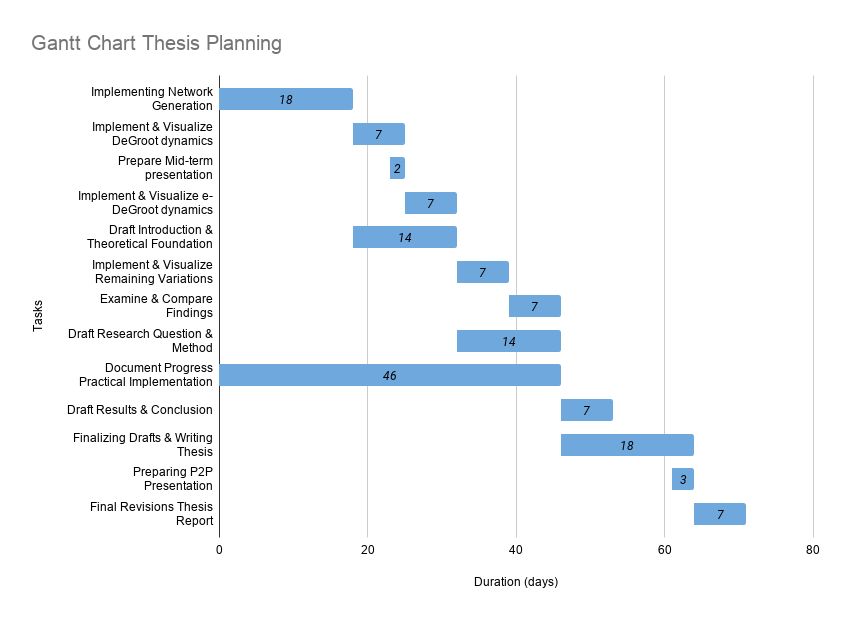
\includegraphics[width=1.2\textwidth]{Gantt2.png}
    \end{figure}
\end{center}

\bibliographystyle{apalike}
\bibliography{references.bib}

\end{document}
